% Options for packages loaded elsewhere
\PassOptionsToPackage{unicode}{hyperref}
\PassOptionsToPackage{hyphens}{url}
%
\documentclass[
]{article}
\title{Assignment 10}
\author{Durga Pokharel}
\date{18/01/2022}

\usepackage{amsmath,amssymb}
\usepackage{lmodern}
\usepackage{iftex}
\ifPDFTeX
  \usepackage[T1]{fontenc}
  \usepackage[utf8]{inputenc}
  \usepackage{textcomp} % provide euro and other symbols
\else % if luatex or xetex
  \usepackage{unicode-math}
  \defaultfontfeatures{Scale=MatchLowercase}
  \defaultfontfeatures[\rmfamily]{Ligatures=TeX,Scale=1}
\fi
% Use upquote if available, for straight quotes in verbatim environments
\IfFileExists{upquote.sty}{\usepackage{upquote}}{}
\IfFileExists{microtype.sty}{% use microtype if available
  \usepackage[]{microtype}
  \UseMicrotypeSet[protrusion]{basicmath} % disable protrusion for tt fonts
}{}
\makeatletter
\@ifundefined{KOMAClassName}{% if non-KOMA class
  \IfFileExists{parskip.sty}{%
    \usepackage{parskip}
  }{% else
    \setlength{\parindent}{0pt}
    \setlength{\parskip}{6pt plus 2pt minus 1pt}}
}{% if KOMA class
  \KOMAoptions{parskip=half}}
\makeatother
\usepackage{xcolor}
\IfFileExists{xurl.sty}{\usepackage{xurl}}{} % add URL line breaks if available
\IfFileExists{bookmark.sty}{\usepackage{bookmark}}{\usepackage{hyperref}}
\hypersetup{
  pdftitle={Assignment 10},
  pdfauthor={Durga Pokharel},
  hidelinks,
  pdfcreator={LaTeX via pandoc}}
\urlstyle{same} % disable monospaced font for URLs
\usepackage[margin=1in]{geometry}
\usepackage{color}
\usepackage{fancyvrb}
\newcommand{\VerbBar}{|}
\newcommand{\VERB}{\Verb[commandchars=\\\{\}]}
\DefineVerbatimEnvironment{Highlighting}{Verbatim}{commandchars=\\\{\}}
% Add ',fontsize=\small' for more characters per line
\usepackage{framed}
\definecolor{shadecolor}{RGB}{248,248,248}
\newenvironment{Shaded}{\begin{snugshade}}{\end{snugshade}}
\newcommand{\AlertTok}[1]{\textcolor[rgb]{0.94,0.16,0.16}{#1}}
\newcommand{\AnnotationTok}[1]{\textcolor[rgb]{0.56,0.35,0.01}{\textbf{\textit{#1}}}}
\newcommand{\AttributeTok}[1]{\textcolor[rgb]{0.77,0.63,0.00}{#1}}
\newcommand{\BaseNTok}[1]{\textcolor[rgb]{0.00,0.00,0.81}{#1}}
\newcommand{\BuiltInTok}[1]{#1}
\newcommand{\CharTok}[1]{\textcolor[rgb]{0.31,0.60,0.02}{#1}}
\newcommand{\CommentTok}[1]{\textcolor[rgb]{0.56,0.35,0.01}{\textit{#1}}}
\newcommand{\CommentVarTok}[1]{\textcolor[rgb]{0.56,0.35,0.01}{\textbf{\textit{#1}}}}
\newcommand{\ConstantTok}[1]{\textcolor[rgb]{0.00,0.00,0.00}{#1}}
\newcommand{\ControlFlowTok}[1]{\textcolor[rgb]{0.13,0.29,0.53}{\textbf{#1}}}
\newcommand{\DataTypeTok}[1]{\textcolor[rgb]{0.13,0.29,0.53}{#1}}
\newcommand{\DecValTok}[1]{\textcolor[rgb]{0.00,0.00,0.81}{#1}}
\newcommand{\DocumentationTok}[1]{\textcolor[rgb]{0.56,0.35,0.01}{\textbf{\textit{#1}}}}
\newcommand{\ErrorTok}[1]{\textcolor[rgb]{0.64,0.00,0.00}{\textbf{#1}}}
\newcommand{\ExtensionTok}[1]{#1}
\newcommand{\FloatTok}[1]{\textcolor[rgb]{0.00,0.00,0.81}{#1}}
\newcommand{\FunctionTok}[1]{\textcolor[rgb]{0.00,0.00,0.00}{#1}}
\newcommand{\ImportTok}[1]{#1}
\newcommand{\InformationTok}[1]{\textcolor[rgb]{0.56,0.35,0.01}{\textbf{\textit{#1}}}}
\newcommand{\KeywordTok}[1]{\textcolor[rgb]{0.13,0.29,0.53}{\textbf{#1}}}
\newcommand{\NormalTok}[1]{#1}
\newcommand{\OperatorTok}[1]{\textcolor[rgb]{0.81,0.36,0.00}{\textbf{#1}}}
\newcommand{\OtherTok}[1]{\textcolor[rgb]{0.56,0.35,0.01}{#1}}
\newcommand{\PreprocessorTok}[1]{\textcolor[rgb]{0.56,0.35,0.01}{\textit{#1}}}
\newcommand{\RegionMarkerTok}[1]{#1}
\newcommand{\SpecialCharTok}[1]{\textcolor[rgb]{0.00,0.00,0.00}{#1}}
\newcommand{\SpecialStringTok}[1]{\textcolor[rgb]{0.31,0.60,0.02}{#1}}
\newcommand{\StringTok}[1]{\textcolor[rgb]{0.31,0.60,0.02}{#1}}
\newcommand{\VariableTok}[1]{\textcolor[rgb]{0.00,0.00,0.00}{#1}}
\newcommand{\VerbatimStringTok}[1]{\textcolor[rgb]{0.31,0.60,0.02}{#1}}
\newcommand{\WarningTok}[1]{\textcolor[rgb]{0.56,0.35,0.01}{\textbf{\textit{#1}}}}
\usepackage{graphicx}
\makeatletter
\def\maxwidth{\ifdim\Gin@nat@width>\linewidth\linewidth\else\Gin@nat@width\fi}
\def\maxheight{\ifdim\Gin@nat@height>\textheight\textheight\else\Gin@nat@height\fi}
\makeatother
% Scale images if necessary, so that they will not overflow the page
% margins by default, and it is still possible to overwrite the defaults
% using explicit options in \includegraphics[width, height, ...]{}
\setkeys{Gin}{width=\maxwidth,height=\maxheight,keepaspectratio}
% Set default figure placement to htbp
\makeatletter
\def\fps@figure{htbp}
\makeatother
\setlength{\emergencystretch}{3em} % prevent overfull lines
\providecommand{\tightlist}{%
  \setlength{\itemsep}{0pt}\setlength{\parskip}{0pt}}
\setcounter{secnumdepth}{-\maxdimen} % remove section numbering
\ifLuaTeX
  \usepackage{selnolig}  % disable illegal ligatures
\fi

\begin{document}
\maketitle

\hypertarget{create-two-quantitative-variables-age-and-body-mass-index-bmi-with-random-samples-of-size-1000-each}{%
\section{Create two quantitative variables: age and body-mass index
(BMI) with random samples of size 1000
each:}\label{create-two-quantitative-variables-age-and-body-mass-index-bmi-with-random-samples-of-size-1000-each}}

\begin{verbatim}
 * Age: 0 to 99 (random samples)
 * BMI: 10 to 40 (random samples)
 
\end{verbatim}

\texttt{Age}

\begin{Shaded}
\begin{Highlighting}[]
\NormalTok{age }\OtherTok{\textless{}{-}} \FunctionTok{sample}\NormalTok{(}\DecValTok{0}\SpecialCharTok{:}\DecValTok{99}\NormalTok{,}\AttributeTok{size =} \DecValTok{1000}\NormalTok{, }\AttributeTok{replace =}\NormalTok{T)}
\end{Highlighting}
\end{Shaded}

\texttt{BMI}

\begin{Shaded}
\begin{Highlighting}[]
\NormalTok{bmi }\OtherTok{\textless{}{-}} \FunctionTok{sample}\NormalTok{(}\DecValTok{10}\SpecialCharTok{:}\DecValTok{40}\NormalTok{, }\AttributeTok{size =} \DecValTok{1000}\NormalTok{, }\AttributeTok{replace =}\NormalTok{ T)}
\end{Highlighting}
\end{Shaded}

\hypertarget{create-a-binary-variable-sex-1male-and-0female-of-1000-random-samples}{%
\section{Create a binary variable sex (1=Male and 0=Female) of 1000
random
samples}\label{create-a-binary-variable-sex-1male-and-0female-of-1000-random-samples}}

\hypertarget{create-a-data-frame-as-df-containing-four-variablesfeaturesserial-number-bmi-age-and-sex}{%
\section{Create a data frame as df containing four
variables/features:Serial Number, BMI, Age and
Sex}\label{create-a-data-frame-as-df-containing-four-variablesfeaturesserial-number-bmi-age-and-sex}}

\begin{Shaded}
\begin{Highlighting}[]
\NormalTok{sn }\OtherTok{\textless{}{-}} \FunctionTok{c}\NormalTok{(}\DecValTok{1}\SpecialCharTok{:}\DecValTok{1000}\NormalTok{)}
\NormalTok{df }\OtherTok{\textless{}{-}} \FunctionTok{data.frame}\NormalTok{(sn,bmi,age,sex)}
\FunctionTok{head}\NormalTok{(df)}
\end{Highlighting}
\end{Shaded}

\begin{verbatim}
##   sn bmi age sex
## 1  1  17  84   0
## 2  2  34  68   1
## 3  3  20  28   0
## 4  4  31  35   1
## 5  5  29  22   0
## 6  6  28   8   1
\end{verbatim}

\hypertarget{for-replication-of-the-results-use-your-class-roll-number-as-random.seed-during-analysis}{%
\section{For replication of the results, use your class roll number as
random.seed during
analysis}\label{for-replication-of-the-results-use-your-class-roll-number-as-random.seed-during-analysis}}

\hypertarget{split-the-data-into-train-and-test-data-using-80-20-partition}{%
\section{Split the data into ``train'' and ``test'' data using 80-20
partition}\label{split-the-data-into-train-and-test-data-using-80-20-partition}}

\begin{Shaded}
\begin{Highlighting}[]
\FunctionTok{set.seed}\NormalTok{(}\DecValTok{11}\NormalTok{)}
\NormalTok{nd }\OtherTok{=} \FunctionTok{sample}\NormalTok{(}\DecValTok{2}\NormalTok{,}\FunctionTok{nrow}\NormalTok{(df), }\AttributeTok{replace=}\NormalTok{ T,}\AttributeTok{prob =} \FunctionTok{c}\NormalTok{(}\FloatTok{0.8}\NormalTok{,}\FloatTok{0.2}\NormalTok{))}
\NormalTok{train\_data }\OtherTok{\textless{}{-}}\NormalTok{ df[nd }\SpecialCharTok{==}\DecValTok{1}\NormalTok{,]}
\NormalTok{test\_data }\OtherTok{\textless{}{-}}\NormalTok{ df[nd}\SpecialCharTok{==}\DecValTok{2}\NormalTok{, ]}
\end{Highlighting}
\end{Shaded}

\hypertarget{fit-a-linear-regression-model-with-bmi-as-dependent-variable-and-age-and-sex-and-predictors-in-the-train-data-samples}{%
\section{Fit a linear regression model with BMI as dependent variable
and age and sex and predictors in the train data
samples}\label{fit-a-linear-regression-model-with-bmi-as-dependent-variable-and-age-and-sex-and-predictors-in-the-train-data-samples}}

\begin{Shaded}
\begin{Highlighting}[]
\NormalTok{lm1 }\OtherTok{\textless{}{-}} \FunctionTok{lm}\NormalTok{(bmi}\SpecialCharTok{\textasciitilde{}}\NormalTok{.,}\AttributeTok{data =}\NormalTok{ train\_data)}
\FunctionTok{summary}\NormalTok{(lm1)}
\end{Highlighting}
\end{Shaded}

\begin{verbatim}
## 
## Call:
## lm(formula = bmi ~ ., data = train_data)
## 
## Residuals:
##      Min       1Q   Median       3Q      Max 
## -16.9166  -7.8375   0.0367   7.9671  16.4182 
## 
## Coefficients:
##               Estimate Std. Error t value Pr(>|t|)    
## (Intercept) 26.2919588  0.6302516  41.717  < 2e-16 ***
## sn          -0.0031420  0.0007763  -4.047 5.43e-05 ***
## age          0.0012245  0.0078208   0.157    0.876    
## sex          0.8884276  0.4510220   1.970    0.049 *  
## ---
## Signif. codes:  0 '***' 0.001 '**' 0.01 '*' 0.05 '.' 0.1 ' ' 1
## 
## Residual standard error: 9.019 on 1597 degrees of freedom
## Multiple R-squared:  0.0126, Adjusted R-squared:  0.01074 
## F-statistic:  6.79 on 3 and 1597 DF,  p-value: 0.0001507
\end{verbatim}

Here p value grater than 0.05. Hence dependent variable normailly
distributed.

\hypertarget{conduct-residual-analysis-of-the-fitted-model-with-graphs-suggestive-and-tests-confirmative}{%
\section{Conduct residual analysis of the fitted model with graphs
(suggestive) and tests
(confirmative)}\label{conduct-residual-analysis-of-the-fitted-model-with-graphs-suggestive-and-tests-confirmative}}

\texttt{Linearity\ of\ resudial} ** Graphical (Suggestive) **

\begin{Shaded}
\begin{Highlighting}[]
\FunctionTok{plot}\NormalTok{(lm1, }\AttributeTok{which =} \DecValTok{1}\NormalTok{, }\AttributeTok{col=} \FunctionTok{c}\NormalTok{(}\StringTok{"blue"}\NormalTok{))}
\end{Highlighting}
\end{Shaded}

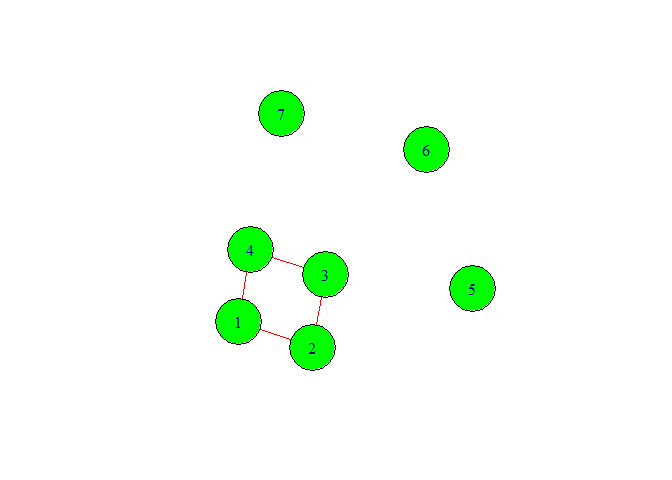
\includegraphics{Assignment-10_files/figure-latex/unnamed-chunk-5-1.pdf}

** Calculation (Confirmative) **

\begin{Shaded}
\begin{Highlighting}[]
\FunctionTok{summary}\NormalTok{(lm1}\SpecialCharTok{$}\NormalTok{residuals)}
\end{Highlighting}
\end{Shaded}

\begin{verbatim}
##      Min.   1st Qu.    Median      Mean   3rd Qu.      Max. 
## -16.91656  -7.83746   0.03668   0.00000   7.96712  16.41823
\end{verbatim}

\texttt{Independence} ** Graphical (suggestive) **

\begin{Shaded}
\begin{Highlighting}[]
\FunctionTok{acf}\NormalTok{(lm1}\SpecialCharTok{$}\NormalTok{residuals)}
\end{Highlighting}
\end{Shaded}

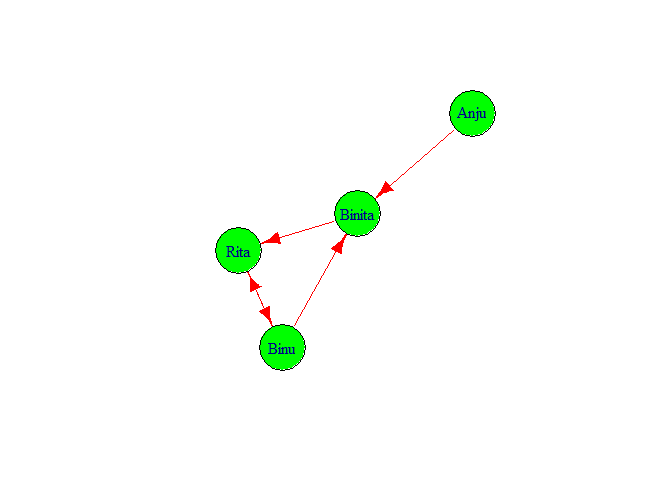
\includegraphics{Assignment-10_files/figure-latex/unnamed-chunk-7-1.pdf}

** Calculatin(Confirmative) **

\begin{Shaded}
\begin{Highlighting}[]
\FunctionTok{library}\NormalTok{(car)}
\FunctionTok{durbinWatsonTest}\NormalTok{(lm1)}
\end{Highlighting}
\end{Shaded}

\begin{verbatim}
##  lag Autocorrelation D-W Statistic p-value
##    1    -0.009230325      2.017583   0.698
##  Alternative hypothesis: rho != 0
\end{verbatim}

\texttt{Normality\ of\ Residuals} ** Graphical(suggestive) **

\begin{Shaded}
\begin{Highlighting}[]
\FunctionTok{plot}\NormalTok{(lm1, }\AttributeTok{which =} \DecValTok{2}\NormalTok{, }\AttributeTok{col =} \FunctionTok{c}\NormalTok{(}\StringTok{"blue"}\NormalTok{))}
\end{Highlighting}
\end{Shaded}

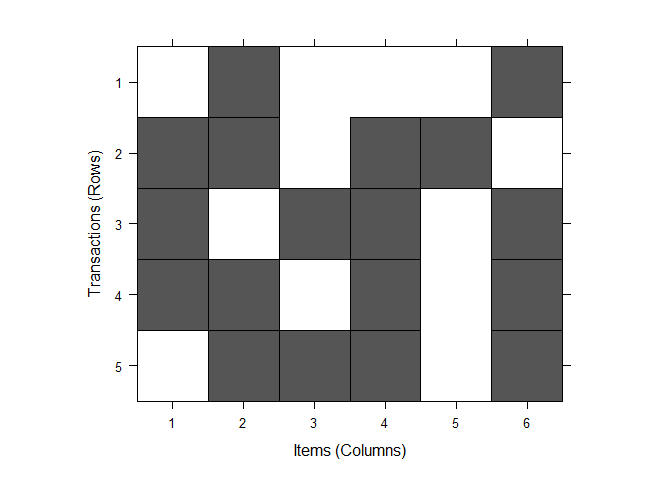
\includegraphics{Assignment-10_files/figure-latex/unnamed-chunk-9-1.pdf}
** Calculation(Confirmative) **

\begin{Shaded}
\begin{Highlighting}[]
\FunctionTok{shapiro.test}\NormalTok{(lm1}\SpecialCharTok{$}\NormalTok{residuals)}
\end{Highlighting}
\end{Shaded}

\begin{verbatim}
## 
##  Shapiro-Wilk normality test
## 
## data:  lm1$residuals
## W = 0.95514, p-value < 2.2e-16
\end{verbatim}

\texttt{Equal\ Variance} ** Graphical(Suggestive) **

\begin{Shaded}
\begin{Highlighting}[]
\FunctionTok{plot}\NormalTok{(lm1,}\AttributeTok{which =} \DecValTok{3}\NormalTok{, }\AttributeTok{col=} \FunctionTok{c}\NormalTok{(}\StringTok{"blue"}\NormalTok{))}
\end{Highlighting}
\end{Shaded}

\includegraphics{Assignment-10_files/figure-latex/unnamed-chunk-11-1.pdf}

** Calculation(Confirmative) **

\begin{Shaded}
\begin{Highlighting}[]
\FunctionTok{library}\NormalTok{(lmtest)}
\end{Highlighting}
\end{Shaded}

\begin{verbatim}
## Loading required package: zoo
\end{verbatim}

\begin{verbatim}
## 
## Attaching package: 'zoo'
\end{verbatim}

\begin{verbatim}
## The following objects are masked from 'package:base':
## 
##     as.Date, as.Date.numeric
\end{verbatim}

\begin{Shaded}
\begin{Highlighting}[]
\FunctionTok{bptest}\NormalTok{(lm1)}
\end{Highlighting}
\end{Shaded}

\begin{verbatim}
## 
##  studentized Breusch-Pagan test
## 
## data:  lm1
## BP = 2.4806, df = 3, p-value = 0.4788
\end{verbatim}

\hypertarget{use-the-fitted-model-to-predict-the-random-test-data-samples}{%
\section{Use the fitted model to predict the random test data
samples}\label{use-the-fitted-model-to-predict-the-random-test-data-samples}}

\begin{Shaded}
\begin{Highlighting}[]
\NormalTok{pred }\OtherTok{\textless{}{-}} \FunctionTok{predict}\NormalTok{(lm1, }\AttributeTok{data =}\NormalTok{ test\_data)}
\FunctionTok{length}\NormalTok{(pred)}
\end{Highlighting}
\end{Shaded}

\begin{verbatim}
## [1] 1601
\end{verbatim}

\begin{Shaded}
\begin{Highlighting}[]
\FunctionTok{length}\NormalTok{(test\_data}\SpecialCharTok{$}\NormalTok{bmi)}
\end{Highlighting}
\end{Shaded}

\begin{verbatim}
## [1] 399
\end{verbatim}

\hypertarget{get-r-square-mse-and-rmse-for-training-as-well-as-test-data-and-interpret-them-carefully}{%
\section{Get R-square, MSE and RMSE for training as well as test data
and interpret them
carefully}\label{get-r-square-mse-and-rmse-for-training-as-well-as-test-data-and-interpret-them-carefully}}

\begin{Shaded}
\begin{Highlighting}[]
\FunctionTok{library}\NormalTok{(}\StringTok{\textquotesingle{}caret\textquotesingle{}}\NormalTok{)}
\end{Highlighting}
\end{Shaded}

\begin{verbatim}
## Warning: package 'caret' was built under R version 4.1.2
\end{verbatim}

\begin{verbatim}
## Loading required package: ggplot2
\end{verbatim}

\begin{verbatim}
## Loading required package: lattice
\end{verbatim}

\begin{Shaded}
\begin{Highlighting}[]
\FunctionTok{data.frame}\NormalTok{(}\AttributeTok{R2 =} \FunctionTok{R2}\NormalTok{(pred, }
\NormalTok{train\_data}\SpecialCharTok{$}\NormalTok{bmi),}
\AttributeTok{RMSE =} \FunctionTok{RMSE}\NormalTok{(pred, }
\NormalTok{train\_data}\SpecialCharTok{$}\NormalTok{bmi),}
\AttributeTok{MAE =} \FunctionTok{MAE}\NormalTok{(pred, }
\NormalTok{train\_data}\SpecialCharTok{$}\NormalTok{bmi))}
\end{Highlighting}
\end{Shaded}

\begin{verbatim}
##           R2     RMSE      MAE
## 1 0.01259527 9.007392 7.804598
\end{verbatim}

From this value of r-square only 0.45\% data fit the regression model.
Which is actually low. Similarly values for RMSE and MAE is respectively
8.909007 and 7.745684. It is better to have low error. Also, I have
tried to get value of R2, RMSE and MAE for test data I got error
\texttt{Error\ in\ cor(obs,\ pred,\ use\ =\ ifelse(na.rm,\ "complete.obs",\ "everything"))\ :\ \ incompatible\ dimensions}
I tried to solve but I could not able.

\end{document}
